
Albert et Béatrice ont commencé des leçons de saxophone. Les deux se déplacent vers vous, en jouant la même note, de fréquence \qty{\v{Freq}}{Hz}. Albert marche à une vitesse de \qty{\v{Valb}}{m/s}, Béatrice à une vitesse de \qty{\v{Vbea}}{m/s}, tandis que vous marchez à \qty{\v{Vvous}}{m/s} (voir le schéma pour la direction de ces vitesses). La vitesse du son est de \qty{343}{m/s}. Quelle est la fréquence des battements que vous entendrez ?

\textit{(Tracez un schéma définissant clairement vos variables, justifiez vos choix de signes dans les équations, et expliquez pourquoi il y a un battement).}

\vspace{0.8cm}
\begin{center}
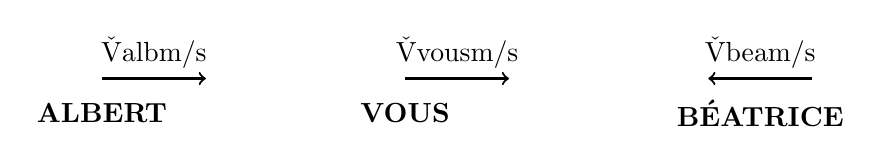
\begin{tikzpicture}[scale=1.1]
    % Albert
    \draw[thick, ->] (0,0) -- (1.2,0) node[midway, above] {\qty{\v{Valb}}{m/s}};
    \node at (0,-0.4) {\textbf{ALBERT}};
    
    % Vous
    \draw[thick, ->] (3.5,0) -- (4.7,0) node[midway, above] {\qty{\v{Vvous}}{m/s}};
    \node at (3.5,-0.4) {\textbf{VOUS}};
    
    % Béatrice
    \draw[thick, <-] (7,0) -- (8.2,0);
    \node at (7.6,0.3) {\qty{\v{Vbea}}{m/s}};
    \node at (7.6,-0.4) {\textbf{BÉATRICE}};
\end{tikzpicture}
\end{center}
\vspace{0.8cm}